\section{Anforderungen}

\subsection{Allgemeine Beschreibung}

\subsubsection{Produktperspektive}


\subsubsection{Produktfunktionen}


\subsubsection{Benutzer Charakteristik}


\subsubsection{Einschränkungen}



\subsection{Use Cases}

\subsubsection{Use Case Diagramm}
\begin{minipage}{\textwidth}

\begin{figure}[H]
	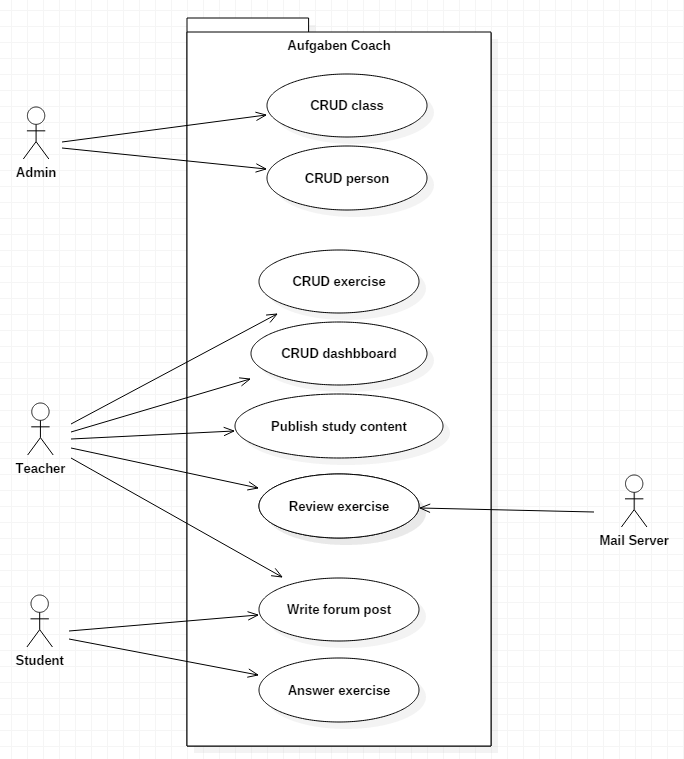
\includegraphics[width=\textwidth, height=\textheight, keepaspectratio]{images/UseCaseDiagramm.png}
	\caption{Use Case Diagramm}
\end{figure}

\end{minipage}



\subsubsection{Aktoren}
Beschreibung der einzelnen Aktoren.
\newline
\begin{tabularx}{\textwidth}{| X | X |}
	\hline
	\textbf{Aktor} & \textbf{Beschreibung} \\
	\hline

	\hline

	\hline
	
	\hline
\end{tabularx}


\subsubsection{Beschreibung der Use Cases}



\subsection{Nicht Funktionale Anforderungen}


\subsubsection{Qualität}


\subsubsection*{Maintainability}


\subsubsection*{Efficiency}


\subsubsection*{Portability}


\subsubsection*{Reliability}


\subsubsection*{Functionality}


\subsubsection*{Usability}


\subsubsection*{Security}


\newpage

\subsubsection{Schnittstellen}

\subsubsection*{Benutzerschnittstellen}

\subsubsection*{Netzwerkschnittstellen}


\newpage